\section{Objectifs, moyens et �valuations}
\leconwithtoc

\subsection{Objectifs}

\begin{frame}{Objectif du cours}
\emph{S'initier � la programmation} au travers de l'apprentissage
\begin{itemize}
\item d'un langage (Java)
\item des bons comportements
  \begin{itemize} 
  \item Programmes lisibles, robustes, document�s et test�s
  \item Capacit�s de \emph{d�verminage} (debugging)
  \item Autonomie dans le travail \\(recherche dans la documentation)
  \end{itemize} 
\end{itemize}
\end{frame}

\begin{frame}{Liens avec les autres cours}
�tapes dans le d�veloppement d'un \textit{Syst�me d'Information}
\begin{center}
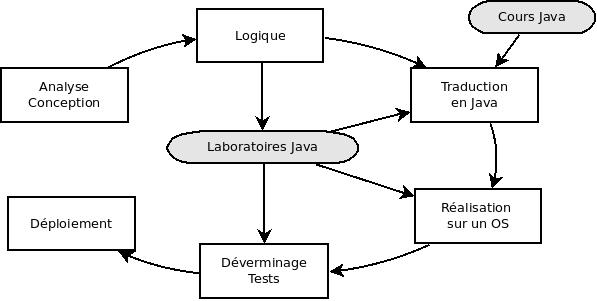
\includegraphics[scale=.5]{../img/etapes-SI} 
\end{center}
\end{frame}

\begin{frame}{Objectif secondaire}
Familiarisation avec le \emph{syst�me d'exploitation} 
(\textit{Operating System})
\emph{Linux}
\begin{itemize}
\item Pas vu au cours
\item Mais utilis� lors des \emph{laboratoires}
\item �tre capable de l'utiliser dans les t�ches courantes de programmation
\end{itemize}
\end{frame}

\subsection{Moyens}

\begin{frame}{Les supports d'apprentissage}
\emph{Pas de syllabus} pour ce cours
\begin{itemize}
  \item De nombreux livres dans le commerce
  \item Les transparents sont disponibles
\end{itemize}
\bigskip
Importance d'un \emph{livre d'accompagnement}
\begin{itemize}
\item Attention : Certains se concentrent sur 
  \begin{itemize}
  \item un aspect bien particulier du langage 
  \item une API sp�cifique
  \end{itemize}
\end{itemize}
\end{frame}

\begin{frame}[fragile]{Les ressources \textit{en ligne}}
De nombreuses ressources sur \emph{po�SI} 
\begin{itemize}
\item la \emph{plateforme d'apprentissage} de l'�SI
\item \code|elearning.esi.heb.be|
\item On y trouve : notes de cours, r�f�rences, \dots
\end{itemize}
\bigskip
Voir aussi le \emph{forum}
\begin{itemize}
\item \code|fora.namok.be|
\item Consult� par des professeurs et des �l�ves
\item Permet
  \begin{itemize}
  \item de se tenir au courant des derni�res nouvelles
  \item d'aider ou de se faire aider en cas de probl�me
  \end{itemize}
\end{itemize}
\end{frame}

\begin{frame}{Le probl�me de l'anglais}
Une connaissance de l'\emph{anglais technique} est \\primordiale
\begin{itemize}
\item Messages d'erreurs 
\item Documentation 
\end{itemize}
\bigskip
Nous essayerons d'introduire chaque nouveau terme dans les deux langues.
\end{frame}

\subsection{�valuations}

\begin{frame}{L'�valuation}
Deux \emph{cotes diff�rentes}
\begin{itemize}
\item Une pour la partie \emph{cours}
\item Une autre pour la partie \emph{laboratoire}
\end{itemize}
\bigskip
\warning{On peut donc r�ussir une partie et pas l'autre.}
\end{frame}

\begin{frame}{L'�valuation du cours}
Uniquement un \emph{oral} en fin d'ann�e
\\\bigskip
Qu'est-ce qu'on attend de vous ?
\begin{itemize}
\item \emph{Comprendre} les concepts abord�s au cours 
 \\ (\emph{pas} de \emph{<<par coeur>>})
\item Pouvoir les expliquer clairement
\item Pouvoir les illustrer au travers d'exemples courts
\item De la \emph{rigueur} : pas d'<<� peu pr�s>>
\item Du \emph{d�tail} : ne pas s'arr�ter � l'<<usage courant>>
\end{itemize}
\end{frame}

\begin{frame}{L'�valuation des laboratoires}
\emph{�valuations continues} pendant les laboratoires
\begin{itemize}
\item Courtes interrogations en \emph{d�but de s�ance}
\item Interrogations de \emph{synth�se}
\item Un \emph{projet}
\end{itemize}
\bigskip
Un examen en fin d'ann�e permet de \emph{remettre en jeu} la cote d'ann�e.
\\\bigskip
Qu'est-ce qu'on attend de vous ?
\begin{itemize}
\item De la \emph{rigueur}
\item De l'\emph{autonomie}
\end{itemize}
\end{frame}
